{
\subsection{Eksperimentsopstilling}
I \ref{chap_afproevning} er de optimale tærskelværdier fundet.
Idet denne hypotese blot kigger på frekvensen for brug af det gyldnesnit
mod andre snit, hvis eneste restriktion er at de skal have et fælles
forhold til det gyldnesnit.
Det er også fordelagtigt at maksimere antallet af andre snit, da det
giver et bedre grundlag for eksperimentet.
Afstanden mellem to snit er begrænset af margin defineret til at være
$2.4\%$\ref{margin}. 
Denne margin skal være tilstede på begge sider af et snit, så derfor vil
hvert snit fylde $(2.4*2)\%$.
Det maksimale antal af snit på et billede må altså være
$100/4.8=20.833$. Hvilket ses på denne figur \ref{snitogmargin}
\begin{figure}[ht]
	\begin{center}
		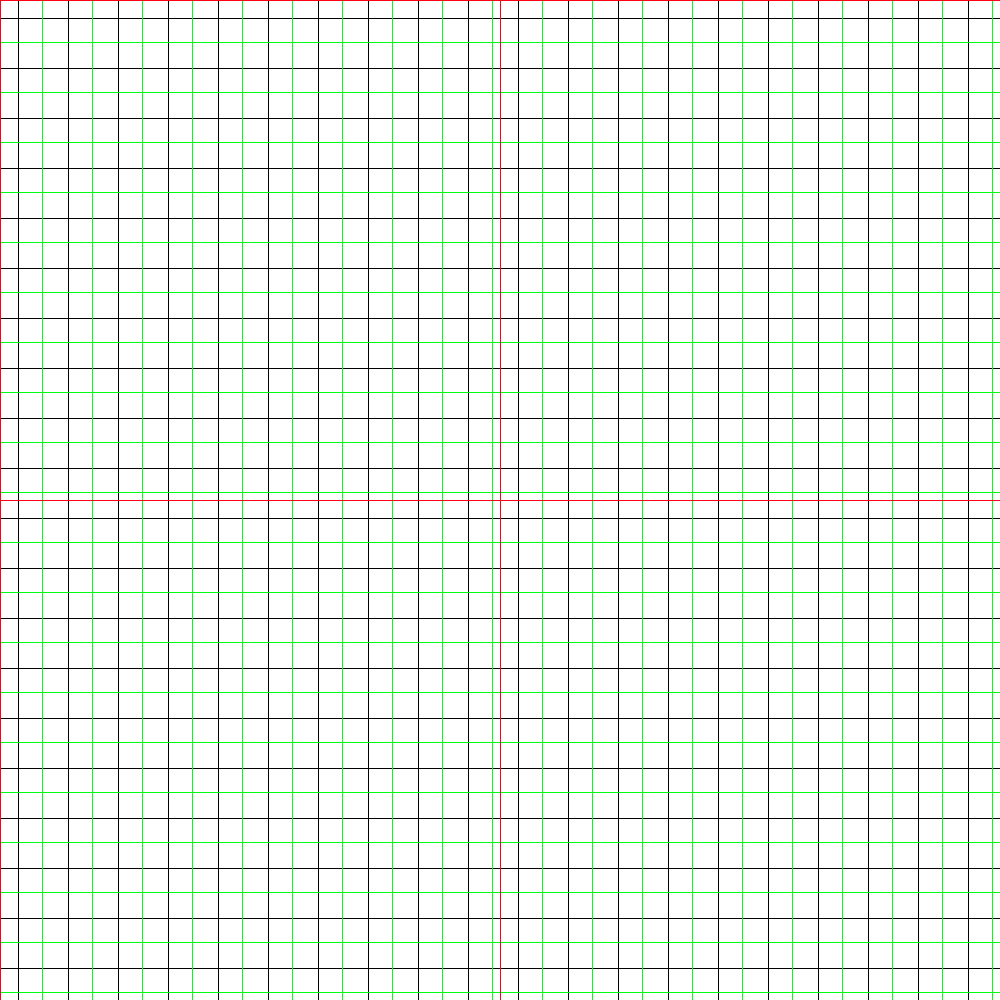
\includegraphics[scale=0.3]{afsnit/resultater/billeder/20_cuts_med_margin}
	\end{center}
	\caption{Sort:snittene, grøn: margins og rød er midten}
	\label{snitogmargin}
\end{figure}
Yderpunkterne $0.958$ og $0.518$ er problematiske, $0.958$'s margin
løber udover billedet, dvs. at den ren principielt går glip af at
detektere en masse interessante regioner.
$0.518$ lider af det modsatte problem, den kan potentielt fange
interessante regioner, på begge sider af midten.
For at være helt præcis så er det i $0.518$ tilfælde:\\
$1-0.518 = 0.482$
$0.518-0.482=0.036$\\
Hvilket er afstanden mellem de to snit.
Der er altså en stimmel på $0.05-0.036 = 0.014 = 1.4\%$ af billedet,
hvor interessante regioner bliver talt to gange.

\subsection{Resultater}
Vi har kørt vores analyse på $17,364$ billeder, men i vores resultater
sorterer vi $2,989$ af disse fra, da de kun er udsnit af et større maleri.
Som vist i tabel \ref{tabel_fjern_detaljer} herunder, er dette en nedgang
på $17.21$ procent og vi har $14,375$ brugbare resultater tilbage.

\begin{table}[H]
    \centering
    \begin{tabular}{r@{\ \ }p{12em}r|r@{.}l}
            & Analyserede malerier & $17,364$ & $100$ & $00\%$   \\
        $-$ & Udsnit af malerier   &  $2,989$ &  $17$ & $21\%$   \\\hline
            & Resultater           & $14,375$ &  $82$ & $79\%$
    \end{tabular}
    \caption[]{Udregning af brugbare resultater.}
    \label{tabel_fjern_detaljer}
\end{table}

Af de brugbare resultater, ser vi i tabel \ref{tabel_fordeling}, at der
i $91.43$ procent af malerierne er fundet mindst én region som ligger i
det gyldne snit. Vi kan derfor ikke afvise hypotese \ref{hypo_binaer}.

\begin{table}[H]
    \centering
    \begin{tabular}{r@{\ \ }p{12em}r|r@{.}l}
            & Positive resultater   & $13,143$ &  $91$ & $43\%$ \\
        $+$ & Negative resultater   &  $1,232$ &   $8$ & $57\%$ \\\hline
            & Resultater i alt      & $14,375$ & $100$ & $00\%$
    \end{tabular}
    \caption[]{Et positivt resultat beskriver et maleri, hvori der er
    fundet mindst én region, som ligger i det gyldne snit. Et negativt
    resultat er et maleri, hvori der ikke findes nogen regioner, som
    ligger i det gyldne snit.}
    \label{tabel_fordeling}
\end{table}

Vi undersøger nu, hvor mange af de brugbare resultater, som er forsynet
med dimensioner i databasen, så vi kan undersøge om lærredet er
konstrueret som et gyldent rektangel. Udregningen i tabel
\ref{tabel_med_dimensioner} viser, at af de brugbare resultater, mangler
$2,410$ denne information og vi har således $11,965$ malerier tilbage at
undersøge for det gyldne rektangel i lærredets dimensioner.

\begin{table}[H]
    \centering
    \begin{tabular}{r@{\ \ }p{14em}r|r@{.}l}
            & Resultater                     & $14,375$ & $100$ & $00\%$ \\
        $-$ & Resultater uden dimensioner    &  $2,410$ &  $16$ & $77\%$ \\\hline
            & Resultater med dimensioner     & $11,965$ &  $83$ & $23\%$
    \end{tabular}
    \caption[]{Brugbare resultater med dimensioner.}
    \label{tabel_med_dimensioner}
\end{table}

Vi ser nu, hvor mange af de $11,965$ malerier, har at dets lange side,
$L$, divideret med dets korte side, $K$, ligger i intervallet $G =
[1.57920117302, 1.65686680448] = \varphi \pm 2.4\%$. Tabel
\ref{tabel_real_dimensions} viser at kun $3.99\%$ falder inden for
dette interval. Vi kan således ikke bekræfte hypotese
\ref{hypo_golden_ractangle}.

\begin{table}[H]
    \centering
    \begin{tabular}{r@{\ \ }p{14em}r|r@{.}l}
            & $L/K \in G$                  &    $478$ &   $3$ & $99\%$ \\
        $+$ & $L/K \notin G$               & $11,487$ &  $96$ & $01\%$ \\\hline
            & Resultater med dimensioner   & $11,965$ & $100$ & $00\%$
    \end{tabular}
    \caption[]{Resultater med dimensioner, hvor disse er et gyldent
    rektangel med en afvigelse på $2.4\%$.}
    \label{tabel_real_dimensions}
\end{table}


%\newpage
%Resultaterne strider ikke mod hypotesen, dog tegner \ref{diffratios}
%et meget et interessante billede. Det er kun de to snit der ligger
%tættere på midten, der indeholder flere interessante regioner.
%Antallet af interessante regioner stiger forholdvis konstant mellem
%$0.77$ og op til $0.57$.

%Med den nuværende algoritme og billedebase burde det gyldnesnit
%altså ligge mellem $0.56803398875 +- 2.4\%$.
%Og tyder meget på at midten langt mere er stedet kunstrene arbejder
%ud fra.
\begin{figure}[ht]
	\begin{minipage}[b]{0.5\linewidth}
		\begin{center}
		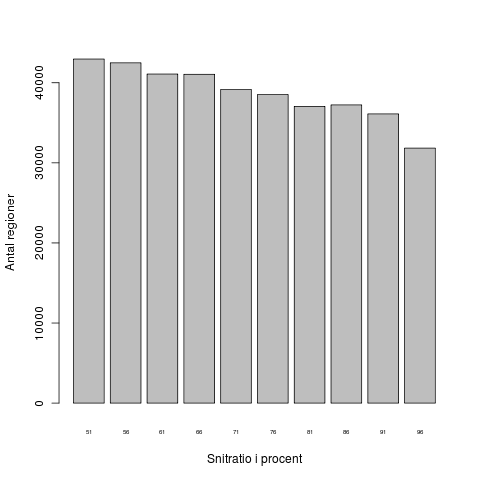
\includegraphics[scale=0.4]{afsnit/resultater/billeder/cut0featsperratio.png}
		\caption{Antal af detekterede interessante regioner i det højre
		vertikale snit}
		\label{cut0feats}
		\end{center}
	\end{minipage}
	\hspace{0.5cm}
	\begin{minipage}[b]{0.5\linewidth}
		\begin{center}
		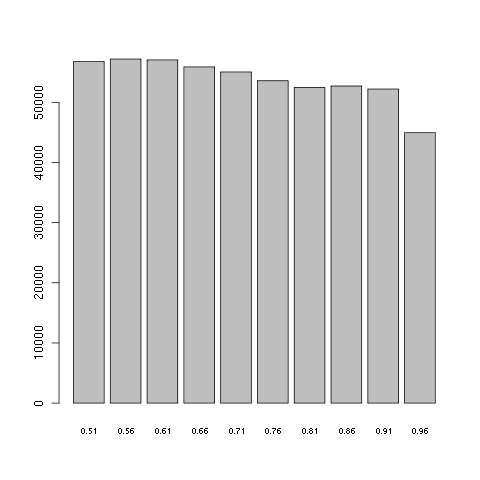
\includegraphics[scale=0.4]{afsnit/resultater/billeder/cut1featsperratio.png}
		\caption{Antal af detekterede interessante regioner i det
		venstre vertikale snit}
		\label{cut1feats}
		\end{center}
	\end{minipage}
\end{figure}
\begin{figure}[ht]
	\begin{minipage}[b]{0.5\linewidth}
		\begin{center}
		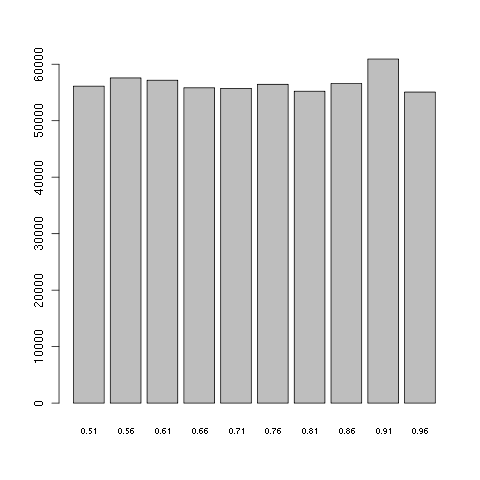
\includegraphics[scale=0.4]{afsnit/resultater/billeder/cut2featsperratio.png}
		\caption{Antal af detekterede interessante regioner i det højre
		vertikale snit}
		\label{cut0feats}
		\end{center}
	\end{minipage}
	\hspace{0.5cm}
	\begin{minipage}[b]{0.5\linewidth}
		\begin{center}
		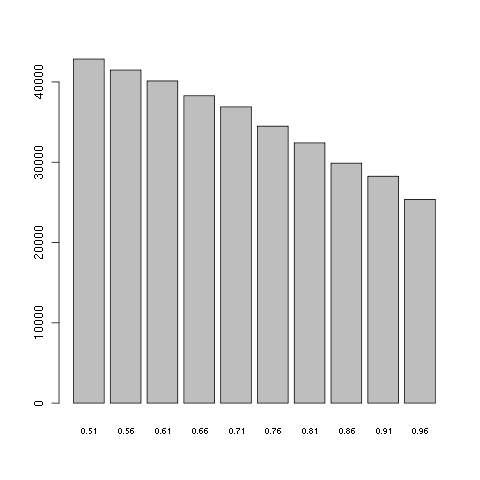
\includegraphics[scale=0.4]{afsnit/resultater/billeder/cut3featsperratio.png}
		\caption{Antal af detekterede interessante regioner i det
		venstre vertikale snit}
		\label{cut1feats}
		\end{center}
	\end{minipage}
\end{figure}

\begin{figure}[h!]
	\begin{center}
		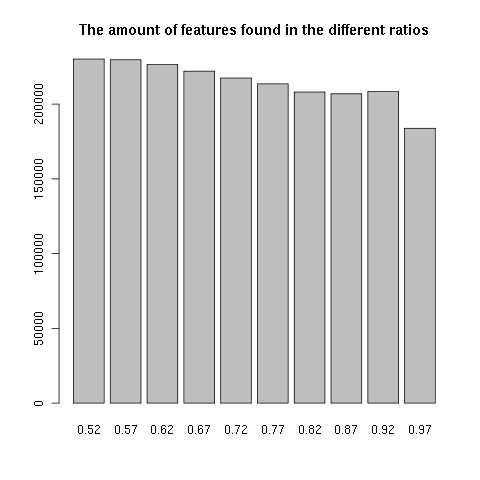
\includegraphics[scale=0.5]{afsnit/resultater/billeder/featsperratio.png}
	\end{center}
	\caption{Antal af detektere interessante regioner på de forskellige snit.}
	\label{diffratios}
\end{figure}




%\begin{verbatim}
%number of features in the golden ratio in different periodes
%
%{'1301-1350\r\n': 151894, '1551-1600\r\n': 184246, '1201-1250\r\n': 419, '1851-1900\r\n': 15092, '1101-1150\r\n': 2817, '1651-1700\r\n': 171119, '1351-1400\r\n': 35464, '1251-1300\r\n': 11864, '1451-1500\r\n': 428338, '1701-1750\r\n': 115703, '1151-1200\r\n': 14688, '1751-1800\r\n': 67703, '1801-1850\r\n': 79182, '1601-1650\r\n': 273832, '1401-1450\r\n': 199989, '1501-1550\r\n': 394100}
%Which golden ration is the most popular, ranging from 0 to 3
%[56092, 57044, 59181, 54152]
%features in the different ratios
%{0.66803398874999997: 222018, 0.86803398875000004: 206899, 0.56803398875: 229650, 0.96803398875000002: 183833, 0.76803398874999995: 213570, 0.91803398874999997: 208340, 0.81803398875: 208081, 0.71803398875000002: 217432, 0.51803398874999995: 230144, 0.61803398875000004: 226462}
%Top 10 cuts, where the most features was found
%[239, 250, 254, 257, 274, 288, 298, 326, 430, 436]
%Top 10 images
%[546, 552, 554, 569, 570, 578, 592, 616, 634, 675]
%Top 10 images, with only the features in the golden feature
%[73, 75, 76, 77, 78, 86, 87, 87, 99, 147]
%Top 10 images, with only features in 2/3 that counts
%[144, 146, 171, 204, 209, 211, 221, 228, 251, 300]
%\end{verbatim}
%TODO:tilføj en ud af hvor mange billeder der var i den periode!
%	og hvilke billeder der er i top 10!
%	og en fordelen af hvor mange features der er i billeder generelt.
%
}
% vim: set tw=72 spell spelllang=da:
